\section{Реализация и тестирование}
Объем написанного кода составляет:
\begin{itemize}
\item 88 Кбайт или 2400 строк на языке C++
\item 22 Кбайт или 670 строк на языке OpenCL C
\item 2 Кбайт или 134 строки на языке cmake
\end{itemize}

Объем измененного кода в заголовочных файлах библиотеки OpenCL, а так же в исходных файлах приложения oclVolumeRender составляет около 200 строк кода на C++.

Объем автоматически сгенерированного кода составляет 3 Кбайта в одном файле.

Тестирование проводилось на последовательности изображений, сгенерированных в программе для трехмерного моделирования Blender. Данные о матрицах калибровки изображений так же брались из программы. Эти данные загружались в программу qcovc и запускался алгоритм. Проверка верности результата проводилась вручную путем визуального сравнения полученной вокселной модели с исходными изображениями.

Пример изображения из исходной последовательности представлен на рисунке ниже.

\begin{figure}[h]
\center
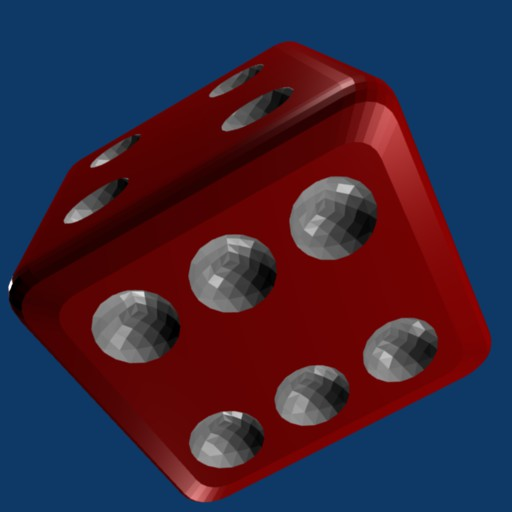
\includegraphics[scale=0.5]{input}
\caption{Изображение из исходной последовательности}
\end{figure}

Увеличение производительности алгоритма составило около 10 \% от реализации на CPU. Для сравнения программа была собрана с использованием фреймворка FOXC~\cite{foxc}, который позволяет выполнять программы, написанные на языке OpenCL C, на центральном процессоре компьютера, что можно считать эквивалентым полному выполнению алгоритма на центральном процессоре.

